\documentclass{article}
\setlength{\parskip}{5pt} % esp. entre parrafos
\setlength{\parindent}{0pt} % esp. al inicio de un parrafo
\usepackage{listings} % listings
\usepackage{color} %colores
\usepackage{amsmath} % mates
\usepackage[sort&compress,numbers]{natbib} % referencias
\usepackage{url} % que las URLs se vean lindos
\usepackage[top=15mm,left=20mm,right=20mm,bottom=25mm]{geometry} % margenes
\usepackage{hyperref} % ligas de URLs
\usepackage{graphicx} % poner figuras
\usepackage[spanish]{babel} % otros idiomas

\author{Claudia Lizeth Hern\'andez Ram\'irez} % author
\title{Homework 5 - M\'etodo Monte-Carlo} % titulo
\date{\today}

\definecolor{mypink}{rgb}{0.976, 0.462, 0.847}
\definecolor{mygray}{rgb}{0.976, 0.980, 0.980}
\definecolor{myblue}{rgb}{0.258, 0.682, 1}
\definecolor{mypink2}{rgb}{0.525, 0.054, 0.4}
\lstset{ 
  backgroundcolor=\color{mygray},
  commentstyle=\color{myblue},
  keywordstyle=\color{mypink}, 
  numberstyle=\tiny\color{mypink}
  stringstyle=\color{mypink2}, 
  breaklines=true,
}


\begin{document} % inicia contenido

\maketitle % cabecera

% RESUMEEEEEEEEEEEEEEEN
\begin{abstract} % resumen
  \centering
Se identifc\'o que conforme aumenta el grupo, es decir, la cantidad de puntos, la probabilidad de obtener dígitos iguales a los del resultado obtenido en \texttt{Wolfram Alpha} es mayor.
  
\end{abstract}


% INTRODUCCIOOOOOOOOOOOON
\section{Introducci\'{o}n}\label{intro} % seccion y etiqueta

En esta tarea se estudiar\'a la precisi\'on del estimado del integral con en m\'etodo Monte Carlo, comparado con el valor producido por Wolfram Alpha, en t\'erminos del n\'umero de decimales correctos, aumentando el tamaño de muestra.


% DESARROLLOOOOOOOOOOOO
\section{Desarrollo}\label{desarrollo} % Desarrollo de la tarea
Como se explic\'o en la introducci\'on, el prop\'osito de esta tarea es comparar la cantidad de decimales que resultan igual en el valor obtenido de la p\'agina \texttt{Wolfram Alpha} y el que obtenemos del c\'odigo base, que vimos en clase\cite{Cbase}.

Comenc\'e generando un pequeño programa el cu\'al comparar\'ia la cantidad de decimales entre un n\'umero y otro utilizando \texttt{strings}.
\begin{lstlisting}[language=R, caption= C\'odigo para comparar n\'umeros como strings.]

suppressMessages (library(tidyverse))
numewolf = 0.369258147 #numero obtenido de WolframAlpha
numerock  = 0.365257741 #numero obtenido en el programa
as.character(numewolf)
as.character(numerock)
datos = data.frame()

posicion = 3
str_sub(as.character(numewolf), 3, posicion)
str_sub(as.character(numerock), 3, posicion)

while (str_sub(as.character(numewolf), 3, posicion) == 
       str_sub(as.character(numerock), 3, posicion)) {
  print(posicion-2)
  posicion = posicion + 1
}
datos = (rbind(datos, posicion-3))
\end{lstlisting}

Posteriormente, era necesario incluir ese c\'odigo en el que vimos en clase \cite{Cbase}, por lo que era necesario hacer algunos cambios para que pudiera ser compatible; Por mencionar algunos, \texttt{numerock} tomar\'ia el valor del resultado de la integral que arroja el c\'odigo base y \texttt{numewolf = 0.048834}. Estos resultados fueron guardados en una data frame llamado \texttt{compara}

\begin{lstlisting}[language=R, caption= C\'odigo data frame \texttt{compara}.]
while (str_sub(as.character(numewolf), 3, posicion) == 
           str_sub(as.character(numerock), 3, posicion)) {
      print(posicion-2)
      posicion = posicion + 1
    }
    datos = c(i, posicion-3)
    compara = (rbind(compara, datos))
    names(compara) = c("Cantidad", "DecimalesCorrectos")
  }
\end{lstlisting}

Antes de hacer pruebas estad\'isticas es necesario realizar pruebas de normalidad a nuestros datos para decidir la prueba que utilizaremos, en este caso como las muestras no exceden de las 50 repeticiones, utilizaremos la prueba de normalidad de \texttt{Shapiro Wilk}.

\begin{table}[ht]
    \centering
    \caption{Resultados obtenidos de prueba de normalidad de Shapiro.} 
    \begin{tabular}{|c|c|}
    \hline
    W & P  \\
    \hline
    0.9035 & $1.395\times 10^{-11}$ \\
    \hline 
\end{tabular}
    \label{cuadro 1}
\end{table}

\begin{lstlisting}[language=R, caption= C\'odigo prueba de normalidad Shapiro-Wilk.]
#Estadistica Shapiro Wilk
compara
str(compara)
names(compara)
shapiro.test(compara$DecimalesCorrectos)
\end{lstlisting}
Planteando que:


- \texttt{Hip\'otesis nula}: la distribuci\'on de la variable es normal.

- \texttt{Hip\'otesis alternativa}: la distribuci\'on de la variable no es normal.

En la literatura podemos encontrar que diversos autores establecen que en pruebas de normalidad para aceptar la hip\'otesis nula el valor de \texttt{P} debe ser mayor al 0.05, es decir mayor al 5\%. De los resultados mostrados en el cuadro 1, observamos que nuestros valores de \texttt{P} son por mucho, menores a 0.05, por lo tanto tenemos pruebas suficientes para \texttt{rechazar} nuestra hip\'otesis nula.

Ahora, sabiendo que la distribuci\'on de nuestros datos no son \texttt{normales}, que tenemos m\'as de dos grupos por analizar y adem\'as son muestras independientes, trabajaremos con la prueba de \texttt{Kruskal-Wallis}\cite{SeleccionPruebas}.

\begin{table}[ht]
    \centering
    \caption{Resultados obtenidos de prueba Kruskal-Wallis.} 
    \begin{tabular}{|c|c|c|}
    \hline
    Chi cuadrada & DF & P  \\
    \hline
    149.23 & 4 & $2.2\times 10^{-16}$ \\
    \hline
\end{tabular}
    \label{cuadro 2}
\end{table}

\begin{lstlisting}[language=R, caption= C\'odigo prueba estad\'istica Kruskal-Wallis.]
#Estadistica Kruskal Wallis
compara%>%
  group_by(Cantidad) %>%
  summarise(
    promedio = mean(DecimalesCorrectos, na.rm = TRUE),
    desviacion_std = sd(DecimalesCorrectos, na.rm = TRUE),
    varianza = sd(DecimalesCorrectos, na.rm = TRUE)^2,
    mediana = median(DecimalesCorrectos, na.rm = TRUE),
    rango_intercuartil = IQR(DecimalesCorrectos, na.rm = TRUE)
  )

kruskal.test(DecimalesCorrectos ~ Cantidad, data = compara)
pairwise.wilcox.test(compara$DecimalesCorrectos, compara$Cantidad) #diferencias entre grupos
\end{lstlisting}

\begin{table}[ht]
    \centering
    \caption{Diferencias entre grupos. Kruskal-Wallis.} 
    \begin{tabular}{|c|c|c|c|c|}
    \hline
    "" & 5k & 50k & 500k & 5M \\
    \hline
    50k & 0.00037 & "" & "" & "" \\
    \hline
    500k & $1.1\times 10^{-10}$ & 0.00046 & "" & "" \\
    \hline
    5M & $3.2\times 10^{-15}$ & $2.0\times 10^{-9}$ & 0.00076 & "" \\
    \hline
    50M & $2.0\times 10^{-16}$ & $5.0\times 10^{-15}$ & $4.6\times 10^{-10}$ & 0.00038 \\
    \hline
\end{tabular}
    \label{cuadro 3}
\end{table}

Del cuadro \ref{cuadro 3} podemos deducir que existen diferencias estad\'isticamente significativas entre los grupos, lo cual es comprobado visualmente en la figura \ref{Figura 1}.

\begin{figure}[h!] % figura
    \centering
    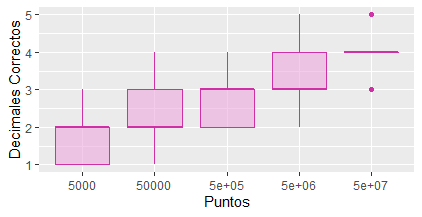
\includegraphics[width=150mm]{boxplothw5.png} % archivo
    \caption{Variaci\'on de la cantidad de decimales correctas respecto al n\'umero de puntos.}
    \label{Figura 1}
\end{figure}

\begin{lstlisting}[language=R, caption= C\'odigo data frame \texttt{compara}.]
# Boxplot
compara$Cantidad = as.factor(compara$Cantidad)
ggplot(compara, aes(x=Cantidad, y=DecimalesCorrectos)) +
  geom_boxplot(fill = "#efa9dd", color = "#cf30a6", alpha = 0.6) +
  labs(x="Puntos", y="Decimales Correctos") 
\end{lstlisting}




%CONCLUSIOOOON
\section{Conclusi\'on}

Teniendo que:

-Hip\'otesis nula: las medias de poblaci\'on son todas iguales.

-Hip\'otesis alternativa: las medias de poblaci\'on no son todas iguales.
y con un nivel de significancia = 0.05. Podemos rechazar la hip\'otesis nula, por lo tanto las diferencias entre algunas medianas son estad\'isticamente significativas.
Se identifc\'o que conforme aumenta el grupo, es decir, la cantidad de puntos, la probabilidad de obtener dígitos iguales a los del resultado obtenido en \texttt{Wolfram Alpha} es mayor.

% BIBLIOGRAFIAAAAAAS
\bibliography{referencias}
\bibliographystyle{plainnat}
\end{document}

